\documentclass[landscape,a0paper,fontscale=0.32]{tikzposter}

% Packages
\usepackage{amsmath}
\usepackage{amssymb}
\usepackage{graphicx}
\usepackage{enumitem}
\usepackage{url}
\usepackage{tikz}
\usetikzlibrary{shapes,arrows,positioning}

% Color theme - Academic
\definecolorstyle{AcademicStyle}{
    \definecolor{colorOne}{RGB}{26,54,93}      % Navy blue
    \definecolor{colorTwo}{RGB}{39,103,73}     % Forest green
    \definecolor{colorThree}{RGB}{247,250,252} % Light gray
}{
    \colorlet{backgroundcolor}{white}
    \colorlet{framecolor}{colorOne}
    \colorlet{titlefgcolor}{white}
    \colorlet{titlebgcolor}{colorOne}
    \colorlet{blocktitlebgcolor}{colorOne}
    \colorlet{blocktitlefgcolor}{white}
    \colorlet{blockbodybgcolor}{colorThree}
    \colorlet{blockbodyfgcolor}{black}
}

\usecolorstyle{AcademicStyle}
\usetitlestyle{Filled}
\useblockstyle{Basic}

% Custom colors
\definecolor{navyblue}{RGB}{26,54,93}
\definecolor{forestgreen}{RGB}{39,103,73}
\definecolor{brickred}{RGB}{197,48,48}
\definecolor{goldaccent}{RGB}{214,158,46}
\definecolor{sensorA}{RGB}{230,126,34}  % Orange for Sensor A
\definecolor{sensorB}{RGB}{52,152,219}   % Blue for Sensor B
\definecolor{lightblue}{RGB}{235,241,250}
\definecolor{lightgreen}{RGB}{235,250,241}
\definecolor{lightred}{RGB}{253,240,240}
\definecolor{lightyellow}{RGB}{255,250,235}
\definecolor{lightorange}{RGB}{253,245,235}
\definecolor{lightgray}{RGB}{245,247,250}

\title{\textbf{Indirect Temperature Estimation Using Kalman Filter (Two Sensors)}}
\author{Probability \& Statistics Course --- Final Project}
\institute{Interactive Demo: \url{https://leonathn.github.io/FinalProjectProbability/}}

\begin{document}

\maketitle

\begin{columns}

%==============================================================================
% COLUMN 1: PROBLEM STATEMENT
%==============================================================================
\column{0.25}

\block{1. The Indirect Measurement Problem}{
\textbf{Goal:} Estimate the true temperature of a light bulb $T_{\text{bulb}}$ that \textbf{cannot be measured directly}.

\vspace{1em}
\innerblock[]{Why Indirect?}{
\begin{itemize}[leftmargin=*,itemsep=0.5em]
    \item Sensors cannot be attached to the hot bulb surface
    \item We can only measure \textbf{air temperature nearby}
    \item Each sensor gives a \textbf{noisy, biased} reading
\end{itemize}
}

\vspace{1em}
\textbf{The Hidden Variable:}
\begin{equation*}
\boxed{T_{\text{bulb}}(k) = \text{True bulb temperature at time } k}
\end{equation*}

\vspace{0.5em}
\textit{This is a classic \textbf{hidden state estimation} problem --- the Kalman Filter's specialty!}
}

\block{2. Two Sensor Setup}{
\vspace{0.5em}
\begin{center}
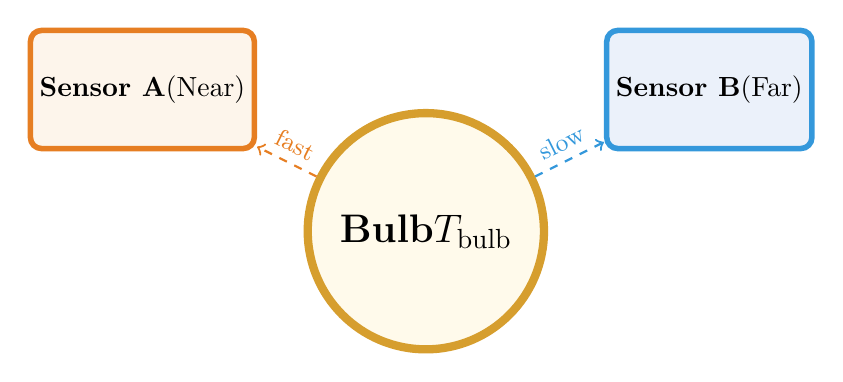
\begin{tikzpicture}[scale=0.9]
    % Bulb
    \node[circle, draw=goldaccent, fill=lightyellow, line width=3pt, minimum size=3cm] (bulb) at (0,0) {\Large\textbf{Bulb}\\$T_{\text{bulb}}$};
    
    % Sensor A - close
    \node[rectangle, draw=sensorA, fill=lightorange, line width=2pt, minimum width=2.5cm, minimum height=1.5cm, rounded corners] (sensorA) at (-4,2) {\textbf{Sensor A}\\(Near)};
    
    % Sensor B - far
    \node[rectangle, draw=sensorB, fill=lightblue, line width=2pt, minimum width=2.5cm, minimum height=1.5cm, rounded corners] (sensorB) at (4,2) {\textbf{Sensor B}\\(Far)};
    
    % Arrows
    \draw[->, thick, sensorA, dashed] (bulb) -- (sensorA) node[midway, above, sloped] {\small fast};
    \draw[->, thick, sensorB, dashed] (bulb) -- (sensorB) node[midway, above, sloped] {\small slow};
\end{tikzpicture}
\end{center}

\vspace{1em}
\innerblock[]{\textcolor{sensorA}{Sensor A} (Near-Bulb Air)}{
\begin{itemize}[leftmargin=*,itemsep=0.3em]
    \item Placed very close to bulb
    \item \textcolor{forestgreen}{\textbf{Fast response}} to temperature changes
    \item \textcolor{brickred}{\textbf{High noise}} ($R_A = 25$), fluctuates a lot
    \item Measures: $z_A = 0.9 \cdot T_{\text{bulb}} + v_A$
\end{itemize}
}

\vspace{0.8em}
\innerblock[]{\textcolor{sensorB}{Sensor B} (Room-Air)}{
\begin{itemize}[leftmargin=*,itemsep=0.3em]
    \item Placed farther in the room
    \item \textcolor{brickred}{\textbf{Slow response}} (thermal lag)
    \item \textcolor{forestgreen}{\textbf{Low noise}} ($R_B = 9$), more stable
    \item Measures: $z_B = 0.6 \cdot T_{\text{bulb}} + v_B$
\end{itemize}
}
}

%==============================================================================
% COLUMN 2: PROBABILISTIC MODEL
%==============================================================================
\column{0.25}

\block{3. State Model (How Temperature Evolves)}{
The bulb temperature follows a random walk with drift:

\vspace{0.8em}
\innerblock[]{State Transition Equation}{
\begin{equation*}
\boxed{T_{\text{bulb}}(k) = T_{\text{bulb}}(k-1) + w_k}
\end{equation*}
where $w_k \sim \mathcal{N}(0, Q)$ is \textbf{process noise}.
}

\vspace{0.8em}
\textbf{Interpretation:}
\begin{itemize}[leftmargin=*,itemsep=0.3em]
    \item Temperature changes slightly each time step
    \item $Q$ = how much we expect it to change (uncertainty)
    \item Small $Q$ = stable temperature, Large $Q$ = volatile
\end{itemize}

\vspace{1em}
\textbf{Example:} $Q = 4$ means temperature might drift by $\pm 2°$C per step on average.
}

\block{4. Measurement Models (What Sensors See)}{
Each sensor observes the hidden temperature \textbf{indirectly}:

\vspace{0.8em}
\innerblock[]{\textcolor{sensorA}{Sensor A Measurement}}{
\begin{equation*}
z_A(k) = H_A \cdot T_{\text{bulb}}(k) + v_A
\end{equation*}
$H_A = 0.9$ (sees 90\% of bulb temp), $v_A \sim \mathcal{N}(0, R_A)$
}

\vspace{0.8em}
\innerblock[]{\textcolor{sensorB}{Sensor B Measurement}}{
\begin{equation*}
z_B(k) = H_B \cdot T_{\text{bulb}}(k) + v_B
\end{equation*}
$H_B = 0.6$ (sees 60\% of bulb temp), $v_B \sim \mathcal{N}(0, R_B)$
}

\vspace{1em}
\textbf{Why Different $H$ Values?}
\begin{itemize}[leftmargin=*,itemsep=0.3em]
    \item $H_A = 0.9$: Sensor A is close, reads almost bulb temp
    \item $H_B = 0.6$: Sensor B is far, air has cooled significantly
\end{itemize}

\vspace{0.8em}
\textbf{Key Insight:} This is \textbf{indirect measurement} --- neither sensor directly reads $T_{\text{bulb}}$!
}

%==============================================================================
% COLUMN 3: KALMAN FILTER EQUATIONS
%==============================================================================
\column{0.25}

\block{5. Scalar Kalman Filter Equations}{
\textbf{No matrices needed!} All equations are simple arithmetic.

\vspace{0.8em}
\innerblock[]{Step 1: Predict State}{
\begin{equation*}
\boxed{\hat{T}^{-}(k) = \hat{T}(k-1)}
\end{equation*}
\centering ``Predicted temperature = previous estimate''
}

\vspace{0.6em}
\innerblock[]{Step 2: Predict Uncertainty}{
\begin{equation*}
\boxed{P^{-}(k) = P(k-1) + Q}
\end{equation*}
\centering ``Uncertainty grows by process noise''
}

\vspace{0.6em}
\innerblock[]{Step 3: Kalman Gain (The Key!)}{
\begin{equation*}
\boxed{K = \frac{H \cdot P^{-}}{H^2 \cdot P^{-} + R}}
\end{equation*}
\centering $K$ = how much to trust this sensor's reading
}

\vspace{0.6em}
\innerblock[]{Step 4: Update Estimate}{
\begin{equation*}
\boxed{\hat{T}(k) = \hat{T}^{-}(k) + K \cdot (z - H \cdot \hat{T}^{-}(k))}
\end{equation*}
\centering ``Correct prediction using measurement''
}

\vspace{0.6em}
\innerblock[]{Step 5: Update Uncertainty}{
\begin{equation*}
\boxed{P(k) = (1 - K \cdot H) \cdot P^{-}(k)}
\end{equation*}
\centering ``Uncertainty decreases after measurement''
}

\vspace{1em}
\textbf{Apply Steps 3-5 for each sensor!}
}

%==============================================================================
% COLUMN 4: EXAMPLE & INTERPRETATION
%==============================================================================
\column{0.25}

\block{6. Numerical Example (One Time Step)}{
\textbf{Given:} $\hat{T} = 80°C$, $P = 16$, $Q = 4$, $z_A = 78$, $z_B = 52$

\vspace{0.5em}
\textbf{Step 1-2: Prediction}
\begin{align*}
\hat{T}^{-} &= 80°C \\
P^{-} &= 16 + 4 = \mathbf{20}
\end{align*}

\textbf{Step 3-5: Update with \textcolor{sensorA}{Sensor A}} ($H_A=0.9$, $R_A=25$)
\begin{align*}
K_A &= \frac{0.9 \times 20}{0.81 \times 20 + 25} = \frac{18}{41.2} = \textcolor{sensorA}{\mathbf{0.437}} \\
\hat{T} &= 80 + 0.437 \times (78 - 72) = \textcolor{sensorA}{\mathbf{82.6°C}} \\
P &= (1 - 0.437 \times 0.9) \times 20 = \mathbf{12.1}
\end{align*}

\textbf{Step 3-5: Update with \textcolor{sensorB}{Sensor B}} ($H_B=0.6$, $R_B=9$)
\begin{align*}
K_B &= \frac{0.6 \times 12.1}{0.36 \times 12.1 + 9} = \frac{7.26}{13.36} = \textcolor{sensorB}{\mathbf{0.543}} \\
\hat{T} &= 82.6 + 0.543 \times (52 - 49.6) = \textcolor{sensorB}{\mathbf{83.9°C}} \\
P &= (1 - 0.543 \times 0.6) \times 12.1 = \mathbf{8.2}
\end{align*}

\vspace{0.5em}
\textbf{Result:} Final estimate $\hat{T} = 83.9°C$, uncertainty reduced from 20 to 8.2!
}

\block{7. The Kalman Gain as Dynamic Trust}{
\begin{center}
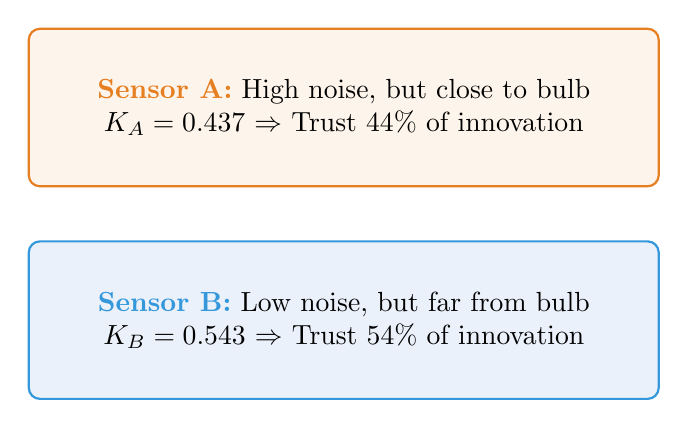
\begin{tikzpicture}[scale=0.9]
    \node[draw=sensorA, thick, fill=lightorange, rounded corners, minimum width=8cm, minimum height=2cm, align=center] at (0,0) {
        \textcolor{sensorA}{\textbf{Sensor A:}} High noise, but close to bulb\\
        $K_A = 0.437$ $\Rightarrow$ Trust 44\% of innovation
    };
    \node[draw=sensorB, thick, fill=lightblue, rounded corners, minimum width=8cm, minimum height=2cm, align=center] at (0,-3) {
        \textcolor{sensorB}{\textbf{Sensor B:}} Low noise, but far from bulb\\
        $K_B = 0.543$ $\Rightarrow$ Trust 54\% of innovation
    };
\end{tikzpicture}
\end{center}

\vspace{0.5em}
\textbf{Weighted Average Interpretation:}
\begin{equation*}
\hat{T}_{\text{new}} = (1-KH) \cdot \hat{T}_{\text{pred}} + K \cdot \frac{z}{H}
\end{equation*}
The filter \textbf{dynamically} balances between prediction and each sensor based on their \textbf{reliability}!
}

\block{8. Conclusion}{
\begin{itemize}[leftmargin=*,itemsep=0.2em]
    \item \textbf{Indirect measurement:} Neither sensor sees true $T_{\text{bulb}}$
    \item \textbf{Sensor fusion:} Combines fast-noisy + slow-stable data
    \item \textbf{Probabilistic:} All based on Gaussian + Bayes
    \item \textbf{Adaptive:} Kalman Gain changes based on uncertainty
\end{itemize}

\vspace{0.5em}
\textbf{Demo:} \url{leonathn.github.io/FinalProjectProbability}
}

\end{columns}

\end{document}
